\section{Implementation}
\subsection{VanillaCase}
\begin{figure}[h]
	\centering
	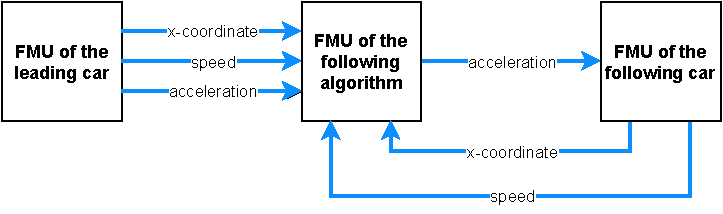
\includegraphics{img/VanillaSchema.pdf}
	\caption{Multi-Model schema del VanillaCase}
\end{figure}

\subsection{Attacco all'accelerazione}
\begin{figure}[h]
	\centering
	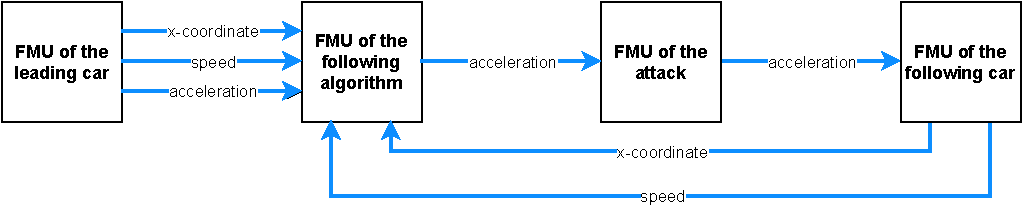
\includegraphics{img/AccelAttackSchema.pdf}
	\caption{Multi-Model schema dell'Attacco alla Accelerazione}
\end{figure}
\subsection{Attacco alla X}
\begin{figure}[h]
	\centering
	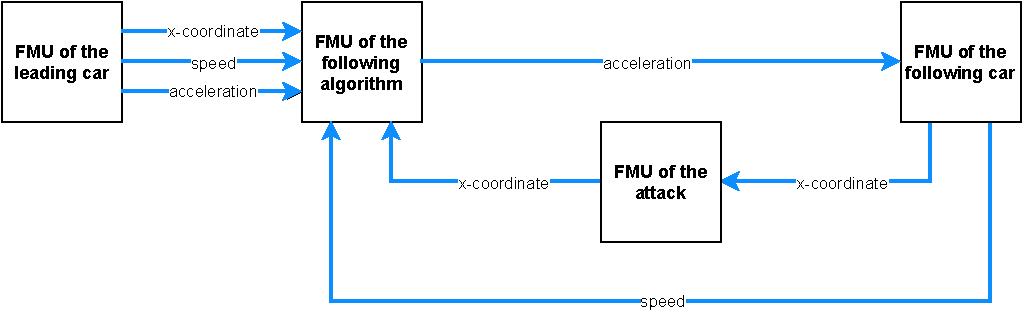
\includegraphics{img/XAttackSchema.pdf}
	\caption{Multi-Model schema dell'Attacco alla X}
\end{figure}
\subsection{Configurazione in Comune}
La configurazione dei seguenti FMU verrà applicata per tutte le simulazioni che verranno effettuate.
\begin{itemize}
	\item \textbf{LeadingCar}:
	\begin{itemize}
		\item Posizione iniziale \textbf{x0}: 50m
		\item Velocità iniziale \textbf{v0}: 0m/s
	\end{itemize}
	
	\item \textbf{FollowingAlgorithm}:
	\begin{itemize}
		\item \textbf{c1}: 1
		\item \textbf{eps}: 0.5
		\item \textbf{omega\_n}: 0.2
	\end{itemize}
	
	
	\item \textbf{FollowingCar}:
	\begin{itemize}
		\item Posizione iniziale \textbf{x0}: 0m
		\item Velocità iniziale \textbf{v0}: 0m/s
	\end{itemize}
\end{itemize}
\subsection{Comportamento degli Attacchi}
L'AttackFMU che verrà utilizzata negli attacchi presenterà due implementazioni diverse:
\begin{itemize}
\item \textbf{Attacco Semplice}: l'attacco consiste nel modificare l'output dell'AttacKFMU con il valore del parametro \textbf{attack\_value} dall'istante temporale \textbf{attack\_time} in poi.
\item \textbf{Attacco Multi-step}: l'attacco consiste nel modificare l'output dell'AttackFMU per un tempo pari a \textbf{attack\_duration}, ripetuto \textbf{attack\_occurrencies} volte e separato nel tempo da \textbf{attack\_distance} secondi. L'attacco inizierà dall'istance temporale \textbf{attack\_time}.

\end{itemize}